% berlin: {"id":"advanced-paper","published":"2026-09-09"}
\documentclass{notebook}
\usepackage{amsmath,amssymb,graphicx,tikz}
\usepackage[hidelinks,pdfusetitle]{hyperref}
\usetikzlibrary{positioning,arrows.meta}
\newcommand{\vect}[1]{\mathbf{#1}}
\title{A Synthetic Dependency Study}
\author{Example Author}
\date{September 9, 2026}
\begin{document}
\maketitle
\begin{abstract}
A synthetic acceptance specimen for multi-file papers, figures, macros and citations.
It makes no research claims.
\end{abstract}
\section{A model}\label{sec:model}
This included section uses a positional macro and the class-defined word \notion{}.
\begin{equation}
\label{eq:vector}
\vect{x} = \begin{bmatrix}1 \\ 2\end{bmatrix}
\end{equation}
Equation~\eqref{eq:vector} remains a numbered, linked expression.

\section{A diagram}\label{sec:diagram}
The \notion{} in Figure~\ref{fig:pipeline} connects the input with its result.
\begin{figure}
\centering
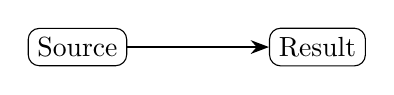
\begin{tikzpicture}[node distance=18mm,>=Stealth]
\node[draw,rounded corners] (source) {Source};
\node[draw,rounded corners,right=of source] (result) {Result};
\draw[->,thick] (source) -- (result);
\end{tikzpicture}
\caption{A directed dependency from the source node to the result node.}
\label{fig:pipeline}
\end{figure}
The two fictional sources are cited together~\cite{example,second}.
An explicit page locator is retained~\cite[p.~7]{example}.
\bibliographystyle{alpha}
\bibliography{references,more}
\end{document}
